%!TEX root = ../dynamics.tex
\section{Analyzing the Features Affecting Batch Throughput}
\label{sec:throughput}
Next, we turn our attention to analyzing the factors that influence the progress (or the pace) of a batch, how those factors influence each other and how their importance changes over time. 

In order to conduct this analysis, we carry out a prediction experiment on the batch's \emph{throughput}, that is, the number of HITs that  will be completed for a given batch within the next time frame of 1 hour (i.e.,  the $DIFF\_HIT$ feature is the target class).
Specifically, we model this task as a regression problem using 29 features; some of them were used in the previous section to classify the HIT type; we describe the remaining ones in Appendix A.

\subsection{Throughput Prediction}

To predict the throughput of a batch at time $T$, we train a Random Forest Regression model with samples taken in the range $[T-\delta, T)$ where $\delta$ is the size of the time window that we are considering directly prior to time $T$. 
%
The rationale behind this approach is that the throughput should be directly correlated to the current and recent market situations. 

In this experiment, we considered  data from June to October 2014, and hourly observations (see Section \ref{sec:tracker}), from which we uniformly sampled 50 time points for evaluation purposes.
%
Our prediction results versus actual throughput values for $\delta=4hours$ are shown in Figure \ref{fig:pred}. 
%
The figure suggests that the prediction works best for larger batches having a large momentum.

In order to understand which features contribute significantly to our prediction model, we proceed by feature ablation. For this experiment, we computed the prediction evaluation score (i.e., R-squared\footnote{\url{http://scikit-learn.org/stable/modules/generated/sklearn.metrics.r2_score.html}}), for 1,000 randomly sampled time points and kept those where the prediction worked reasonably, i.e., having $R^2>0$, that is 327 samples. Next, we rerun the prediction on the same samples by removing one feature at a time. The results revealed that the features $HIT\_available$ (i.e., the number of tasks in the batch) and $Age\_minutes$ (i.e., how long ago the batch was created) were the only ones having a statistically significant impact on the prediction score with $p < 0.05$ and $p < 0.01$ respectively. 

\begin{figure}[t!]
	\centering
		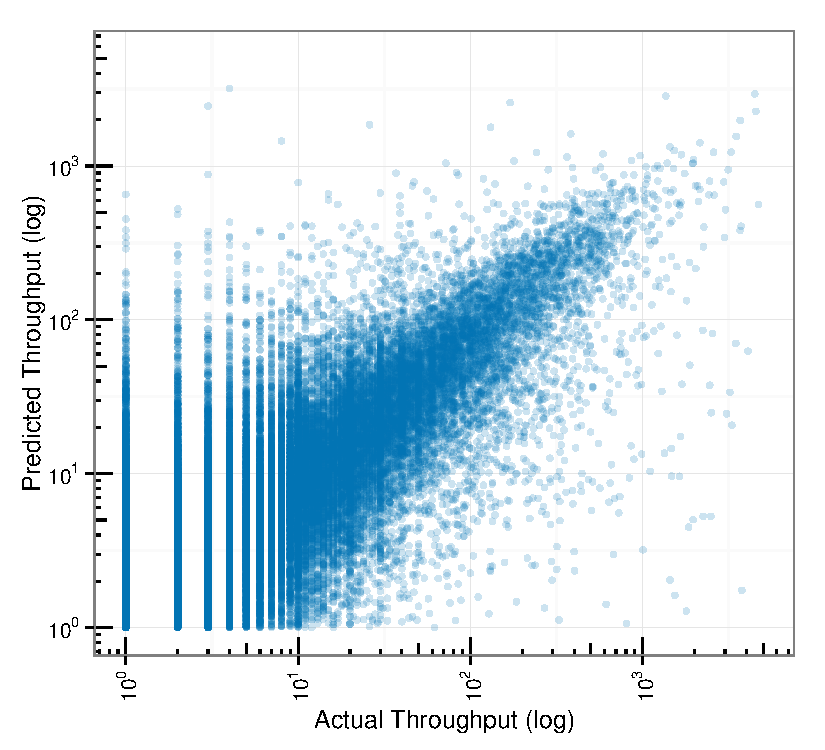
\includegraphics[width=0.45\textwidth]{figures/predictions_3}
	\caption{Predicted vs actual batch throughput values for $\delta=4hours$.}
	\label{fig:pred}
\end{figure}

\subsection{Features Importance}

In order to better grasp the characteristics of the batch throughput, we examine the computed Gini importance of the  features~\cite{breiman}. 
For that, we varied the training time frame $\delta$ from 1 hour to 24 hours for each tested time point. 
Figure \ref{fig:importances} shows the contribution of our 2 top features (as concluded from the previous experiment, i.e., $HIT\_available$ and $Age\_minutes$) and how their importances varied when we increased the training time-frame. These features are again listed in Table \ref{table:feats}, the slope indicates whether the feature is gaining importance over time (positive value) or decreasing in importance (negative value).

The most important feature is $HIT\_available$, that is, the current size of the batch. Indeed, as observed by previous work, larger batches tend to attract more workers \cite{mturk,crowddb}. This feature becomes less important when we consider longer periods, partly because of noise, and because other features start to encode additional facts.
On the other hand, $Age\_minutes$ importance suggests that the crowd is sensitive to newly posted HITs, or how \emph{fresh} the HITs are. 
To better understand this phenomenon, we conduct an analysis on what attracts the workforce to the platform in the next section.

\begin{figure}[t!]
	\centering
		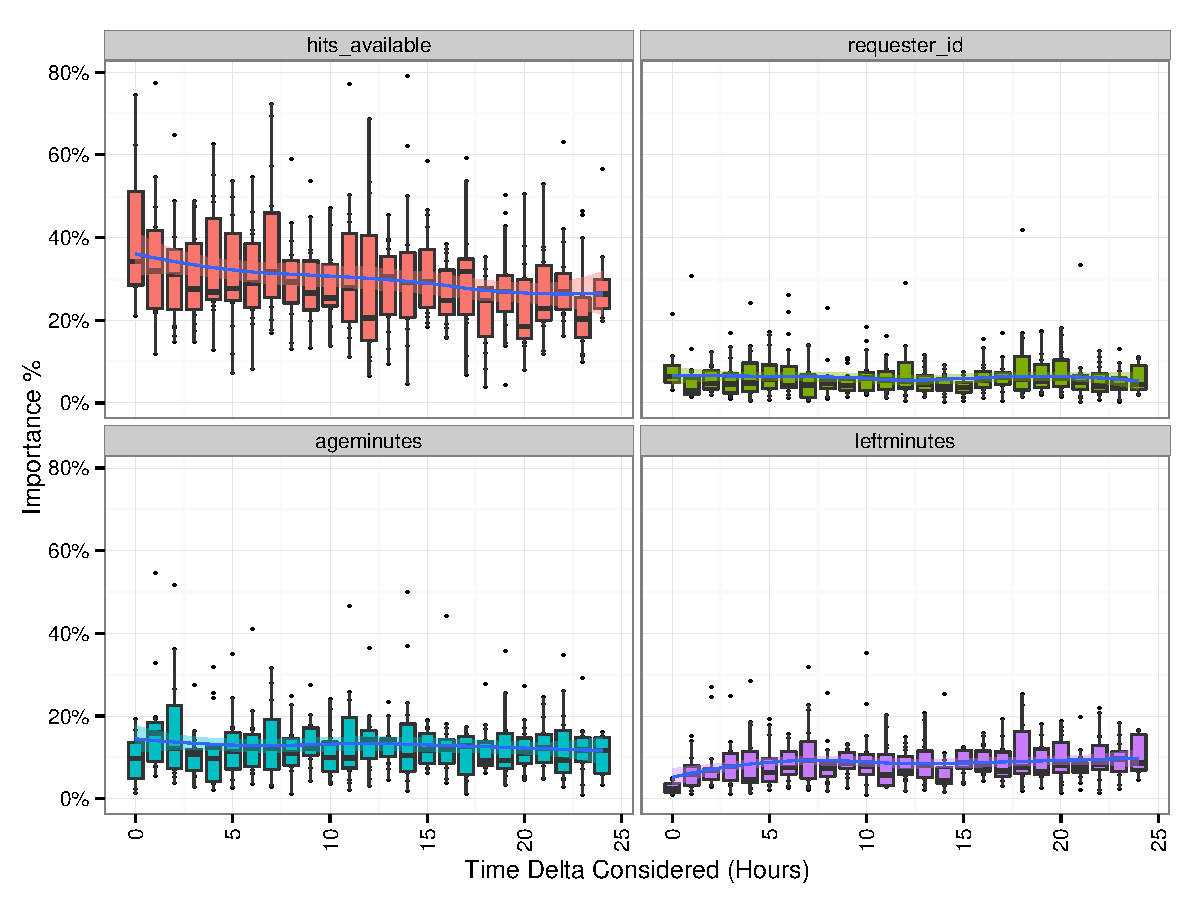
\includegraphics[width=0.5\textwidth]{figures/importances}
	\caption{Computed feature importance when considering a larger training window for batch throughput prediction.}
	\label{fig:importances}
\end{figure}

\begin{table}[t!]
\begin{center}
\scriptsize
\caption {Gini importance of the top 2 features used in the prediction experiment. A large mean indicates a better overall contribution to the prediction. A positive slope indicates that the feature is gaining in importance when the considered time window is larger.}
\begin{tabular}{|c|c|c|c|c|}
\hline
Feature              & mean      & stderr    & slope     & intercept \\
\hline
HIT\_available      & 29.8606 & 13.4247 & -0.0257 & 34.4940 \\
Age\_minutes           & 12.9087 &  8.1967 & -0.0050 & 13.8181 \\
%leftminutes          &  8.7300 &  5.5530 & 0.0061 & 7.6290 \\
%requester\_id        &  6.2147 &  5.2943 & -0.0011 & 6.4305 \\
%title                &  5.6441 &  4.2604 & -0.0033 & 6.2519 \\
%description          &  4.8823 &  3.8975 & -0.0065 & 6.0617 \\
%keywords             &  4.3765 &  3.3860 & -0.0074 & 5.7095 \\
%time\_alloted        &  3.7994 &  3.6820 & -0.0010 & 3.9965 \\
%reward               &  3.5439 &  2.7426 & -0.0011 & 3.7458 \\
%totalapproved        &  2.5259 &  3.5108 & 0.0033 & 1.9311 \\
%tasktype             &  2.1370 &  2.2673 & -0.0008 & 2.2986 \\
%start\_time          &  1.2257 &  1.4123 & 0.0049 & 0.3325 \\
%hitsAvailableUI      &  1.1428 &  1.2062 & 0.0039 & 0.4380 \\
%diffHitsUI           &  1.0557 &  1.1237 & 0.0038 & 0.3568 \\
%hitGroupsAvailableUI &  1.0438 &  1.0219 & 0.0034 & 0.4169 \\
%diffGroupsUI         &  1.0408 &  1.0658 & 0.0030 & 0.4835 \\
%master               &  0.9943 &  2.3816 & -0.0012 & 1.2134 \\
%diffGroups           &  0.9660 &  0.9349 & 0.0032 & 0.3863 \\
%rewardsArrived       &  0.9543 &  1.0710 & 0.0032 & 0.3698 \\
%hitsCompleted        &  0.9293 &  0.9453 & 0.0031 & 0.3593 \\
%percHitsCompleted    &  0.8974 &  0.8548 & 0.0030 & 0.3543 \\
%location             &  0.8957 &  1.7592 & 0.0004 & 0.8184 \\
%diffRewards          &  0.8920 &  0.8967 & 0.0023 & 0.4622 \\
%rewardsCompleted     &  0.8890 &  0.8896 & 0.0026 & 0.4056 \\
%percHitsPosted       &  0.8462 &  0.9552 & 0.0021 & 0.4618 \\
%diffHits             &  0.8462 &  0.7514 & 0.0024 & 0.3972 \\
%hitsArrived          &  0.7562 &  0.7946 & 0.0021 & 0.3760 \\
%approvalrate         &  0.0000 &  0.0000 & 0 & 0 \\
\hline
\end{tabular}
\label{table:feats}
\end{center}
\end{table}